\documentclass[30pt, a0paper, portrait, margin=0mm, innermargin=15mm,
               blockverticalspace=15mm, colspace=15mm, subcolspace=8mm]{tikzposter} 

% Change font     
\renewcommand{\familydefault}{\sfdefault}

\definecolor{mycol}{HTML}{326E77}
\definecolorstyle{myColorStyle}{
  \colorlet{colorOne}{darkgray}
  \colorlet{colorTwo}{gray}
  \colorlet{colorThree}{gray}
}{
  % Background Colors
  \colorlet{backgroundcolor}{colorTwo!50}
  \colorlet{framecolor}{black}
  % Title Colors
  \colorlet{titlefgcolor}{black}
  \colorlet{titlebgcolor}{colorOne}
  % Block Colors
  \colorlet{blocktitlebgcolor}{mycol}
  \colorlet{blocktitlefgcolor}{white}
  \colorlet{blockbodybgcolor}{white}
  \colorlet{blockbodyfgcolor}{black}
  % Innerblock Colors
  \colorlet{innerblocktitlebgcolor}{white}
  \colorlet{innerblocktitlefgcolor}{black}
  \colorlet{innerblockbodybgcolor}{white}
  \colorlet{innerblockbodyfgcolor}{black}
  % Note colors
  \colorlet{notefgcolor}{black}
  \colorlet{notebgcolor}{white}
  \colorlet{notefrcolor}{white}
}

% LATEX PACKAGES
% --------------
  
\usepackage{graphicx}  % package for inserting images, including .pdf
\usepackage{adjustbox} % package for cropping images
\usepackage[colorlinks=true, urlcolor=red]{hyperref} % package for url and hyperlinks
\usepackage{wrapfig}
\usepackage{lmodern} %mix italic and bold
\usepackage{hyperref}% for url
\usepackage{authblk}
\usepackage{graphicx} 
\usepackage{caption}
\usepackage{mwe}
\usepackage[absolute]{textpos}
\usepackage{selinput}
\SelectInputMappings{%
  Lcaron={Ľ}
}


% TITLE, AUTHORS, INSTITUTE
% -------------------------

\title{\textbf{Host-parasite interplay in a mammalian hybrid zone}}

\author[1,2]{Alice~Balard}
\author[1,2]{Victor~Hugo~Jarqu\'{i}n-D\'{i}az}
\author[1]{Jenny~Jost}
\author[3]{Iva~Martincov\'{a}}
\author[3]{{Ľ}udov\'{i}t \v{D}ureje}
\author[3]{Jaroslav~Pi\`alek}
\author[4]{Milo\v{s}~Macholán}
\author[3]{Jo\"{e}lle~Go\"{u}y~de~Bellocq}
\author[3]{Stuart~J.E.~Baird}
\author[1,2]{Emanuel~Heitlinger}
\affil[1]{\Large Institute for Biology. Department of Molecular Parasitology. Humboldt University Berlin (HU). Philippstr. 13, Haus 14, 10115, Berlin, Germany}
\affil[2]{\Large Leibniz-Institut für Zoo- und Wildtierforschung (IZW) im Forschungsverbund Berlin e.V.. Alfred-Kowalke-Straße 17, 10315, Berlin, Germany}
\affil[3]{\Large Research Facility Studenec, Institute of Vertebrate Biology, Czech Academy of Sciences, Kv\v{e}tn\'{a} 8, 603 65 Brno, Czech Republic}
\affil[4]{\Large Laboratory of Mammalian Evolutionary Genetics, Institute of Animal Physiology and Genetics, Czech Academy of Sciences, Veveri 97, 60200 Brno, Czech Republic\vspace{-6ex}% reduce space
}



\makeatletter
\def\maketitle{\AB@maketitle}
\makeatother

% THEME SETTING
% -------------
\usetheme{Default}
\usecolorstyle{myColorStyle}
\useblockstyle{Basic}
\usebackgroundstyle{Empty}
\usetitlestyle{Empty}

% Increase caption size
\usepackage{blindtext}
\makeatletter
\renewenvironment{tikzfigure}[1][]{
  \def \rememberparameter{#1}
  \vspace{10pt}
  \refstepcounter{figurecounter}
  \begin{center}
  }{
    \ifx\rememberparameter\@empty
    \else %nothing
    \\[5pt]
    {\large Fig.~\thefigurecounter: \rememberparameter}
    \fi
  \end{center}
}
\makeatother





% HEAD
% ----

\begin{document}
\maketitle
\begin{columns}

% ------------------------
% COLUMN 1 ---------------

\column{0.5}

% Context
% ----

\block{Context}
{
	\begin{itemize}
	
	  		\item Parasite model: \textit{Eimeria} spp., obligate intracellular parasite (Apicomplexa: Coccidia). \textbf{Three \textit{Eimeria} spp.} identified (3 markers) in the mice of the hybrid zone
	  		 \item Host model: \textit{Mus musculus domesticus}, \textit{Mus musculus musculus}, and hybrids
	
\begin{tikzfigure}[]
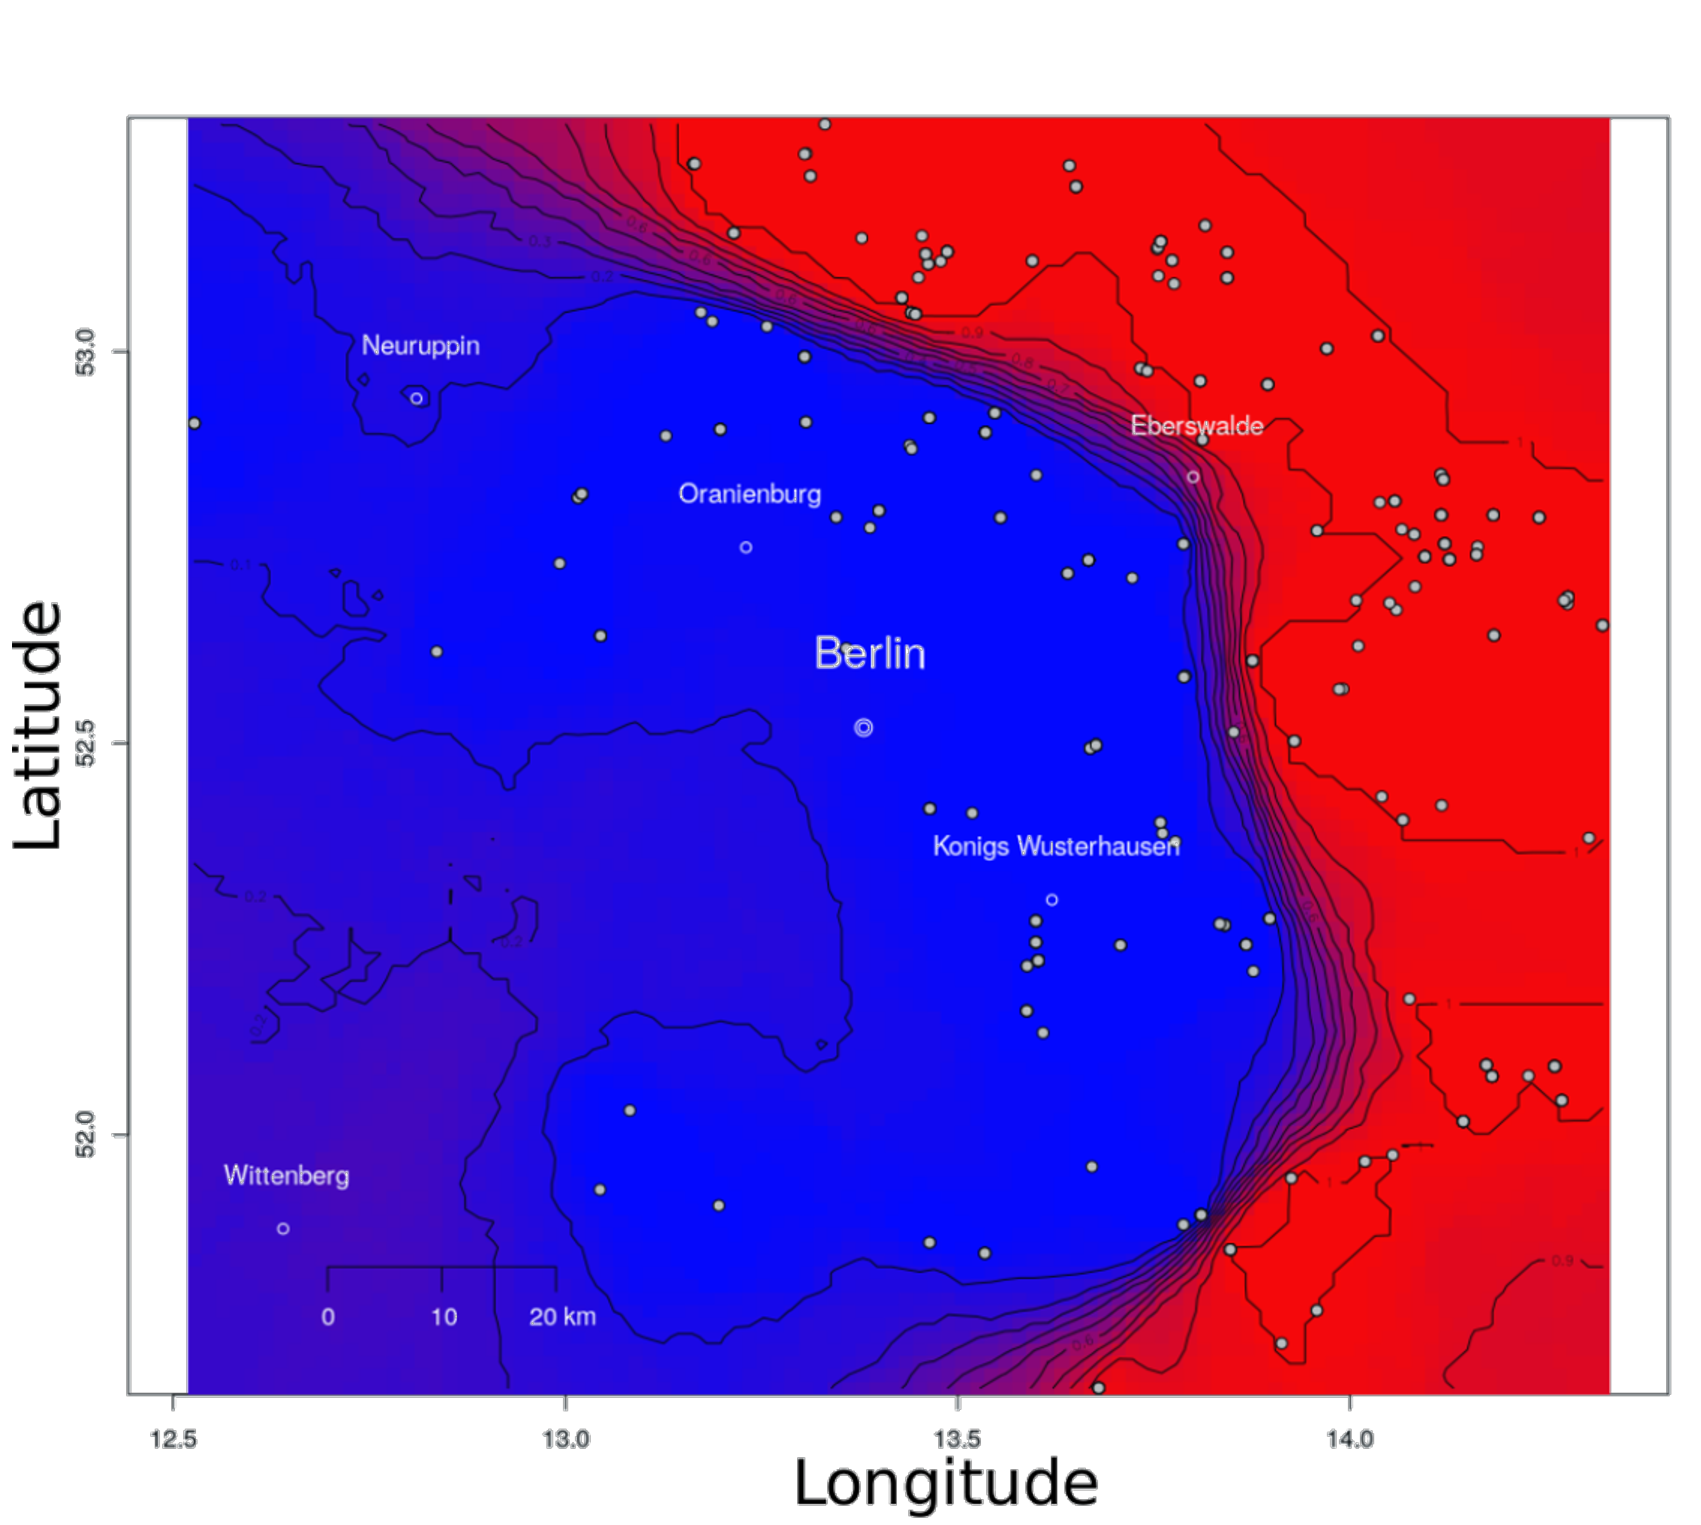
\includegraphics[scale=0.6]{Figure1.pdf}
\end{tikzfigure}
 \textbf{Map of the spatial range of both house mouse subspecies in the European House Mouse Hybrid Zone}. Spatial organization was inferred using six autosomal markers (Es1, H6pd, Idh1, Mpi, Np, Sod1). Mmd is found west of the hybrid zone (blue), Mmm east of it (red). The numbers at the level contours indicate posterior probabilities of population membership for each mouse subspecies
       
        \end{itemize}
}

% AIMS
% ----

\block{Aims of the study}
{
	\begin{enumerate}
	\item Investigate \textbf{hybrid susceptibility/resistance} of house mice to their parasite \textit{Eimeria}~spp. using prevalence and intensity data for parasite strains throughout the House Mouse Hybrid Zone
	\item Compare with pinworms, prevalent but less pathogenic than \textit{Eimeria}~spp
	\end{enumerate}
}


% Material \& Methods
% -------
\block{Material \& Methods}
{

\begin{itemize}
\item Sampling 660 mice over 4 years; Host genotyping (4-14 diagnostic markers) on a 0 to 1 scale (50/50 hybrids = 0.5)
\item \textit{Eimeria} load estimated by quantitative PCR / Pinworm load estimated by count
\item Body condition estimated by residuals body length/body weight

\item Statistical analyses:
      \begin{itemize}
\item Modellisation of parasite load along hybridization index, test hybrid effect
\item Logistic regression presence/absence of parasite in direction of the hybrid zone center
      \end{itemize}
\end{itemize}
    }

% Results: parasite load
% -------

\block{Results: Pinworm load lower in hybrids than in parental mice}
      {
      \begin{tikzfigure}[]
        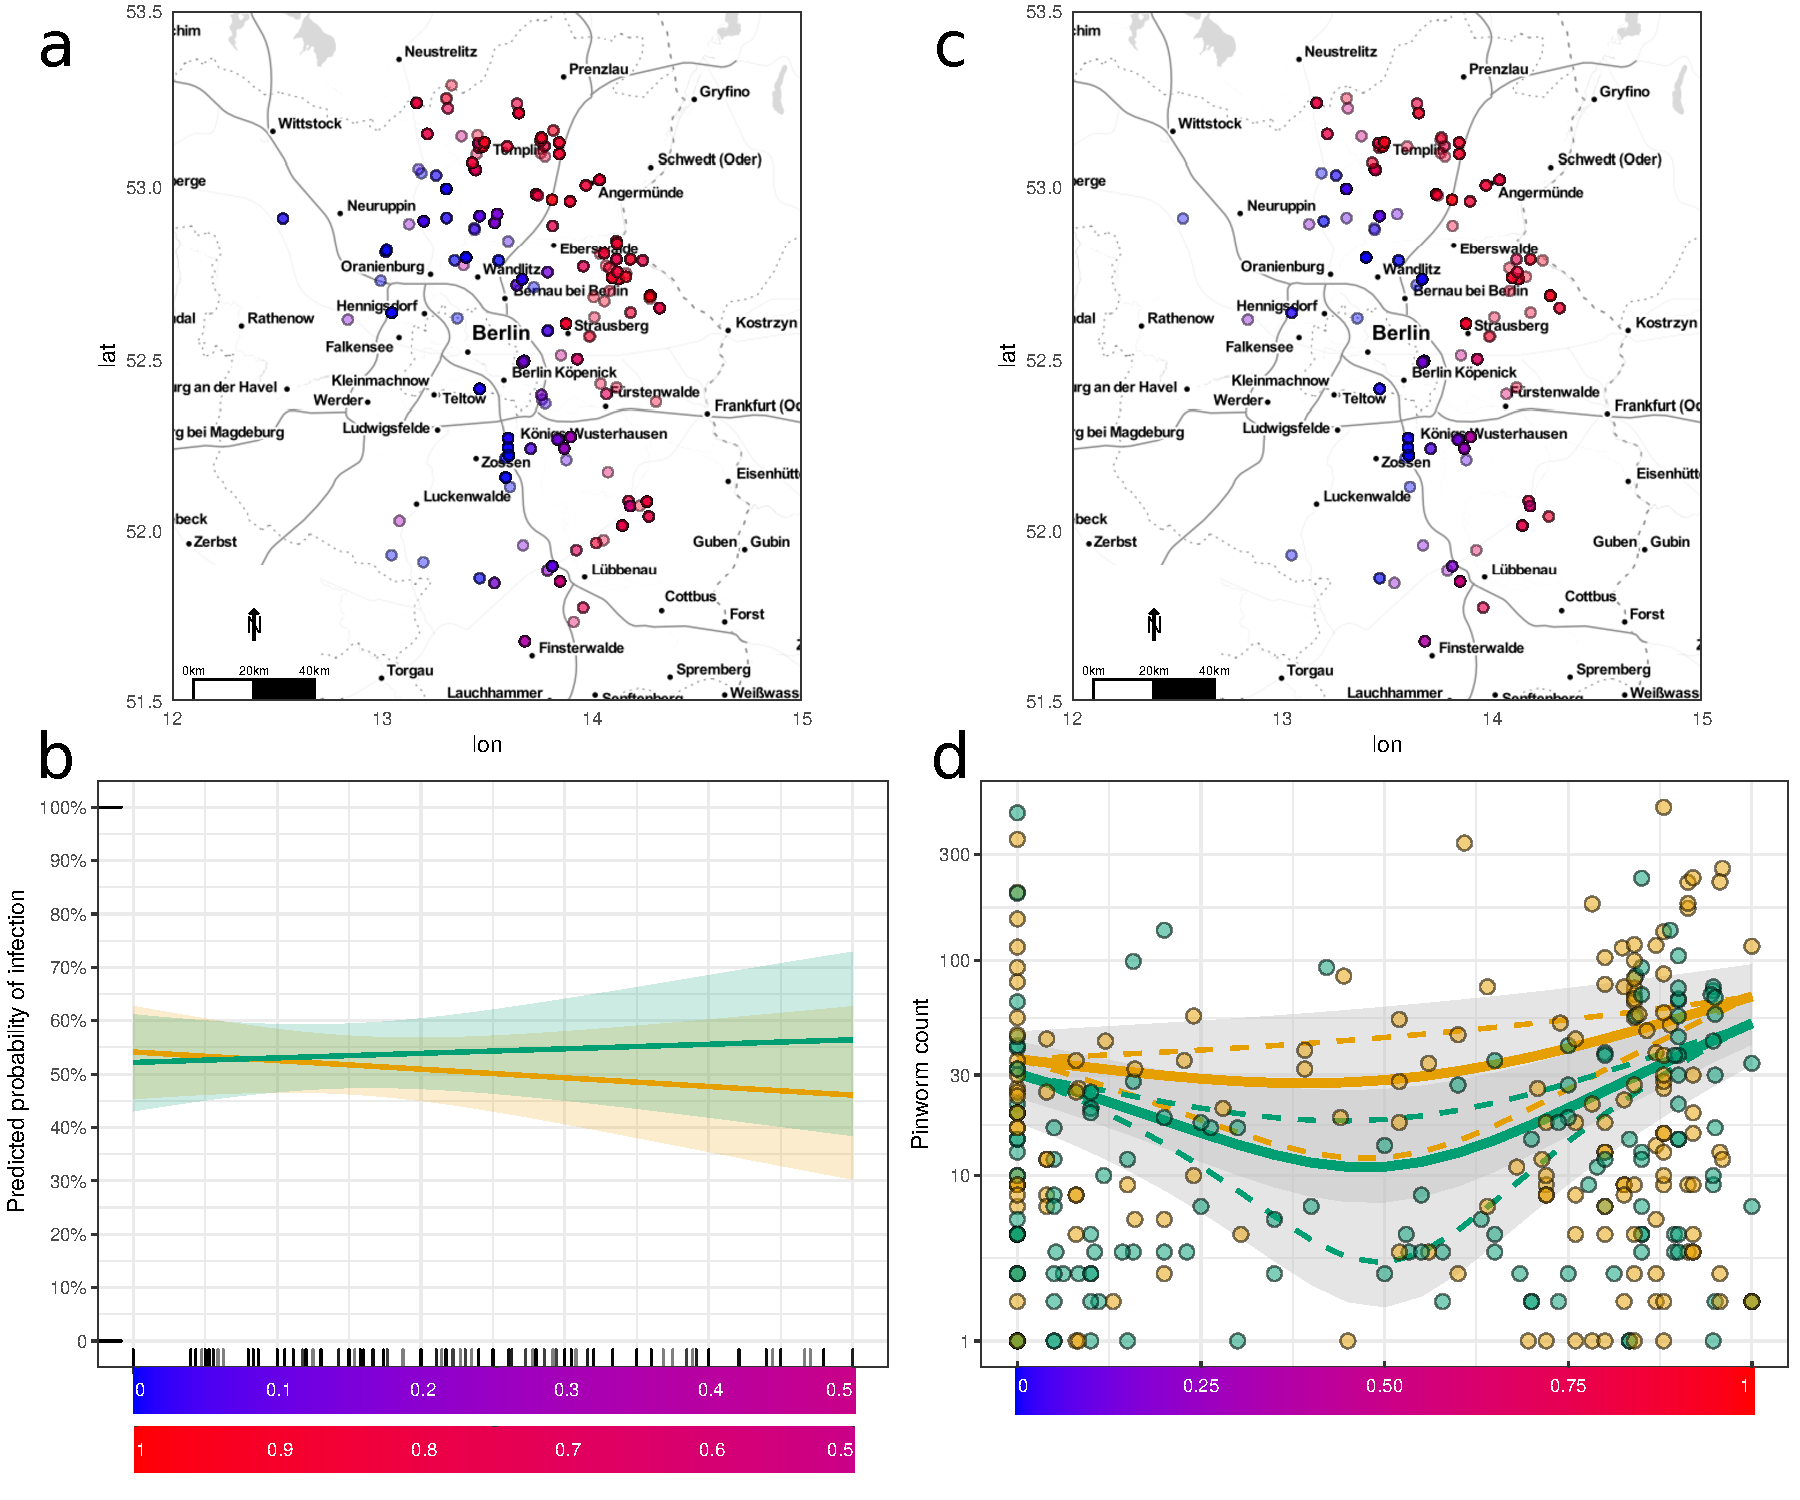
\includegraphics[scale=0.9]{Figure3.pdf}
      \end{tikzfigure}
      Map of all individuals (a), and predicted probability of infection when approaching the hybrid zone center (b). Map of positive individuals (c), and prediction of parasite intensity along the hybrid index (d)(males (green)/females (orange))
}


% ------------------------
% COLUMN 2 ---------------

\column{0.5}

\block{Results: \textit{Eimeria} spp. load lower in hybrids than in parental mice}
      {
     
      \begin{tikzfigure}[]
        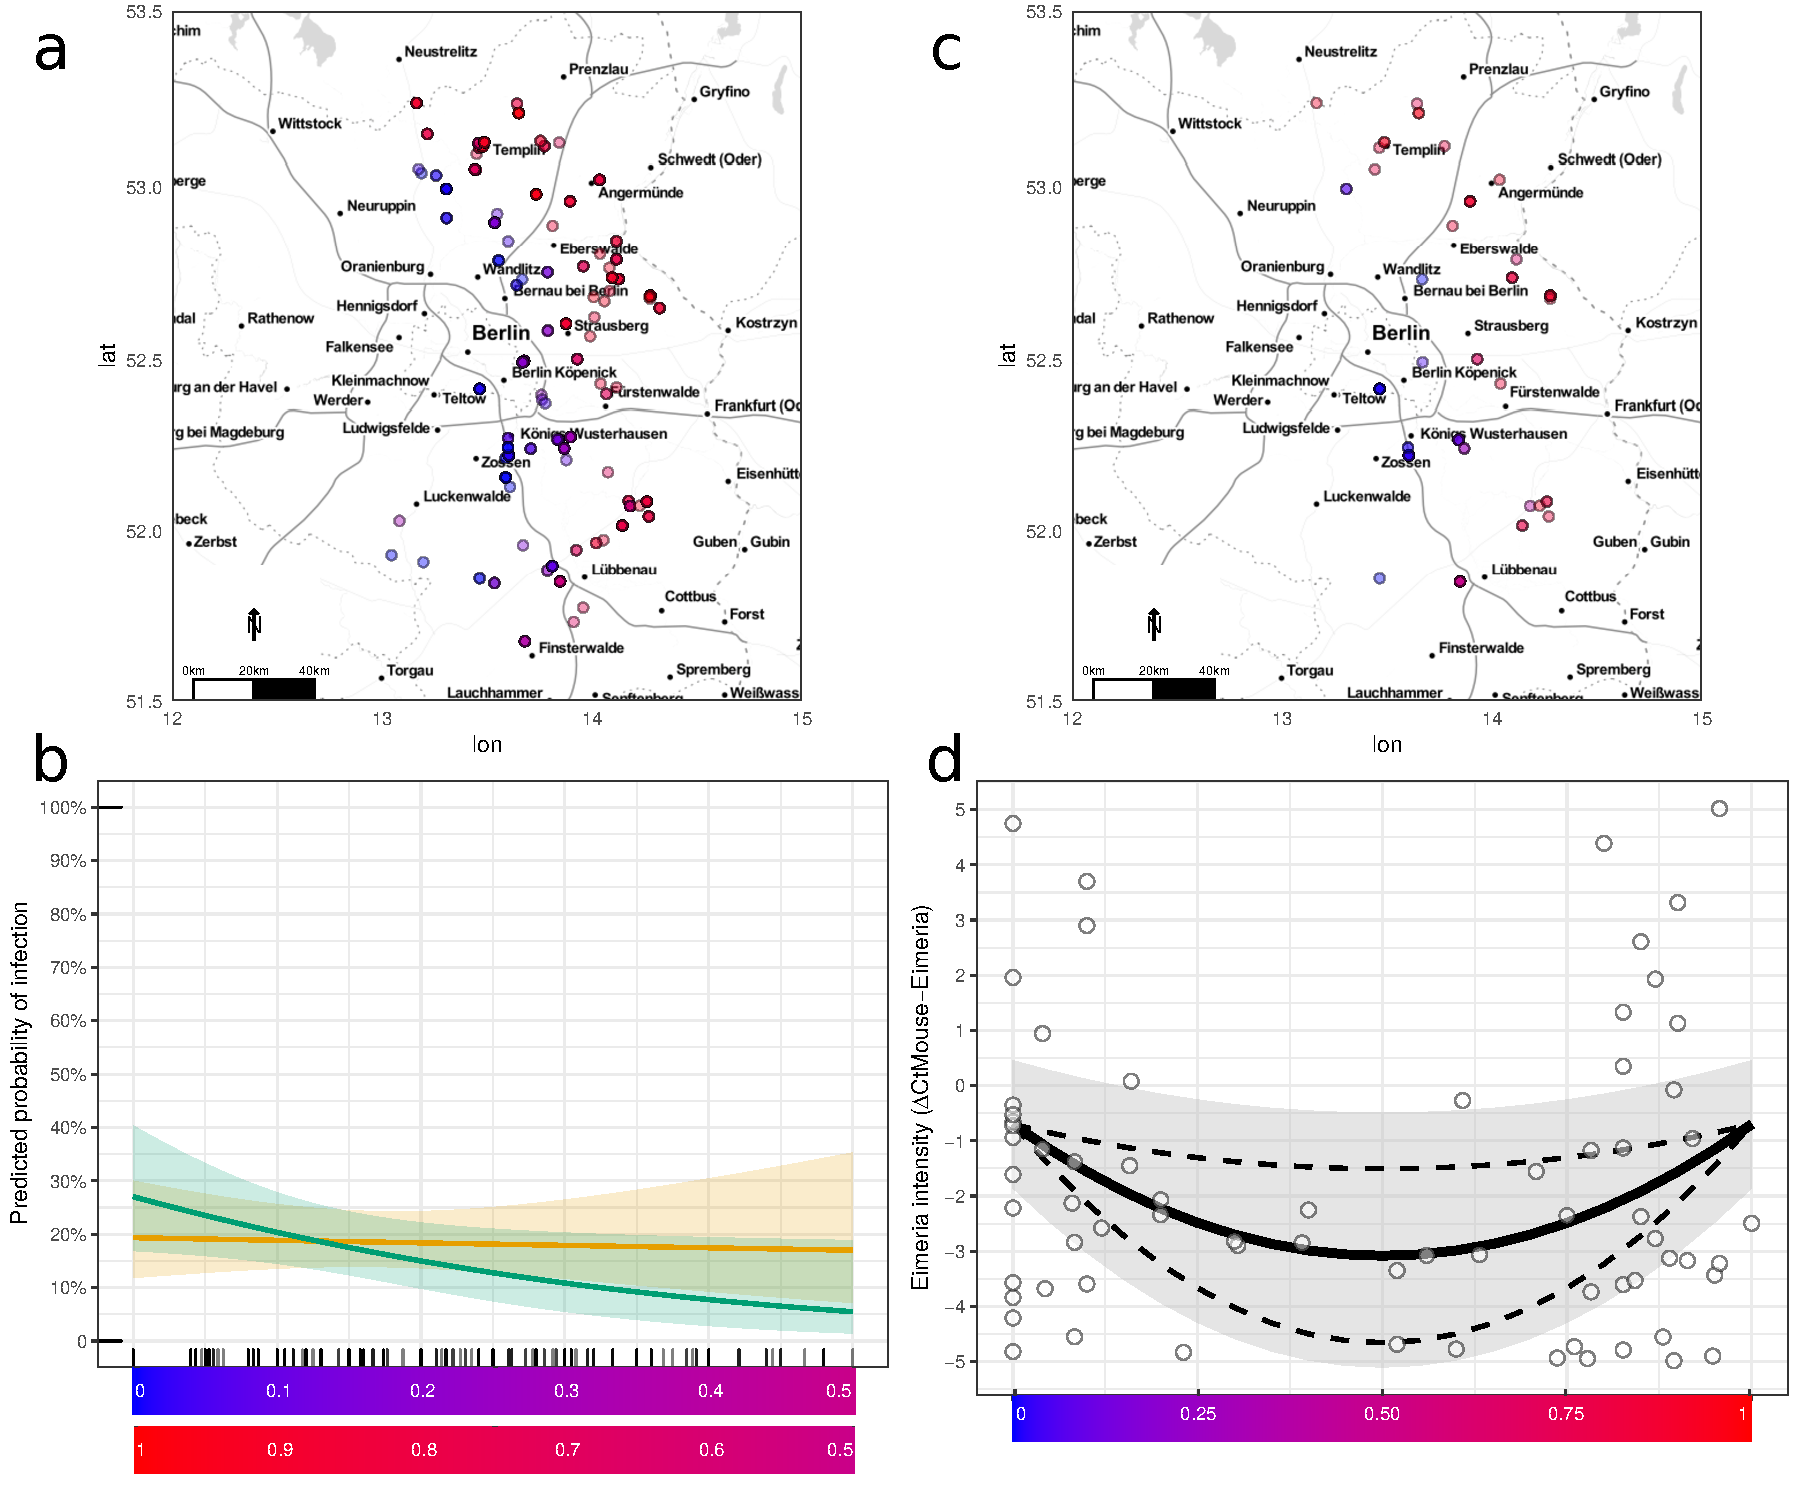
\includegraphics[scale=0.9]{Figure2.pdf}
      \end{tikzfigure}
Map of all individuals (a), and predicted probability of infection when approaching the hybrid zone center (b). Map of positive individuals (c), and prediction of parasite intensity along the hybrid index (d)(males (green)/females (orange))
}

% PART II 
% -------

\block{Results: no indication of differential body condition between infected/non infected}
{ 
\begin{tikzfigure}[]
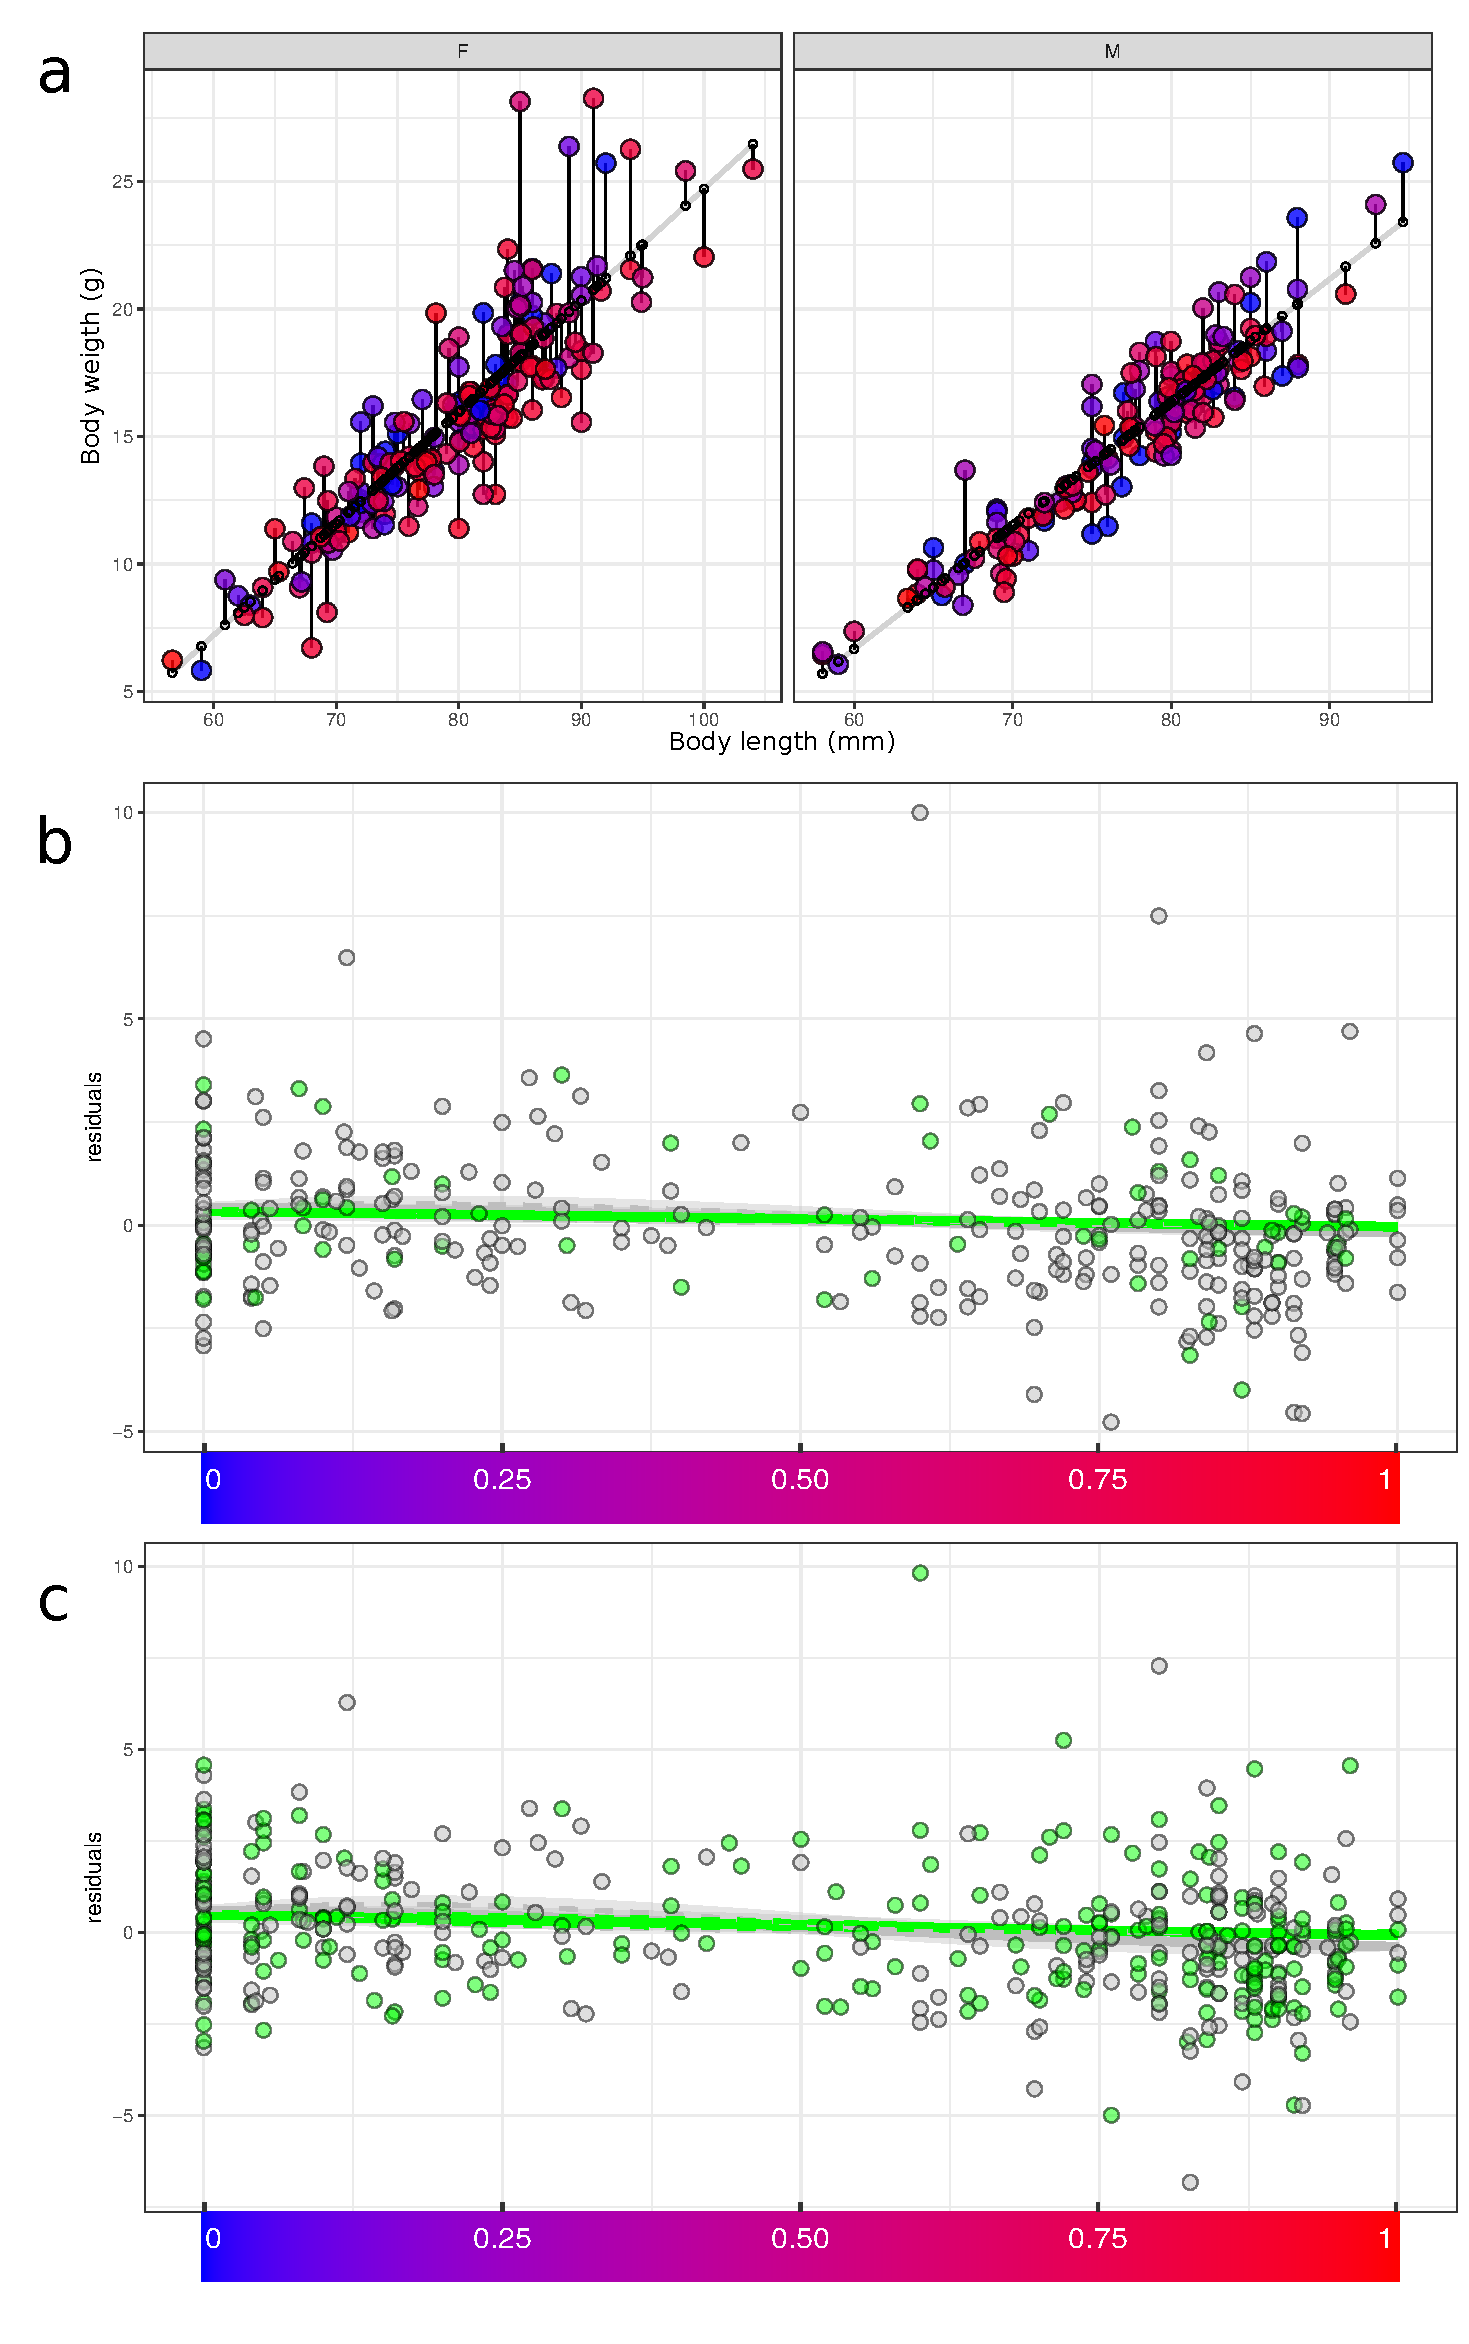
\includegraphics[scale=0.6]{Figure4.pdf}
\end{tikzfigure}
Fit of the residuals for females and males (a); prediction of residuals along the hybrid index (\textit{Eimeria} spp. (b) and pinworms (c)) infected mice (light green) and non infected mice (grey)

}

\block{Conclusion}
{Improving our understanding of parasite process across the HMHZ provides valuable information on the house mouse as the model species with the most thoroughly understood immune system. A transfer of knowledge from this model might help to understand the interplay between parasites and hybridizing species, our own as well as species relevant for conservation.
}

% REFERENCES
% ----------

\block{References}
      {
        \begin{small}
          
          \hangindent=2cm Baird \textit{et al.} (2012) Where Are the Wormy Mice? A Reexamination of Hybrid Parasitism in the European House Mouse Hybrid Zone \textit{Evolution} 66 (9): 2757--72
           
          \hangindent=2cm Heitlinger \textit{et al.} (2014) The genome of Eimeria falciformis-reduction and specialization in a single host apicomplexan parasite \\ \textit{BMC genomics} 15 (1), 696
          
          \hangindent=2cm Machol\'{a}n \textit{et al.} (2011) Assessing Multilocus Introgression Patterns: A Case Study on the Mouse X Chromosome in Central Europe \textit{Evolution} 65: 1428--1446

          \hangindent=2cm Machol\'{a}n \textit{et al.} (2012) Evolution of the House Mouse
          \textit{Cambridge University Press}
          
        
          
        \end{small}
      }

\end{columns}

% ----------------
\end{document}
\endinput
%%
%% End of file 
